%% Use the "review" option when submitting for review.
%% Removing the "review" option will switch the
%% manuscript to a two-column layout.
%%
%% Use option "jog" for submissions to the Journal of
%% Glaciology; use "aog" for submission to the Annals
%% of Glaciology.
\documentclass[aog]{igs}
% \documentclass[review,aog]{igs}

\usepackage[utf8]{inputenc}

\usepackage{mathabx}
\usepackage{graphicx}
\usepackage{siunitx}

% the default is for unnumbered section heads
% if you really must have numbered sections, remove
% the % from the beginning of the following command
% and insert the level of sections you wish to be
% numbered (up to 4):

% \setcounter{secnumdepth}{2}

\jourvolume {1}
\jourissue{1}
\jourpubyear{2024}

\begin{document}

\title[IGS \LaTeXe\ guide]{int != Integer; How choosing the right data type could improve your system's performance}

\author[Baxter and others]{#skill-java@Andela.com,$^1$
  Amuda A,$^2$\protect\thanks{Present address:
  Centre for Glaciology, Institute of Geography and
  Earth Sciences, University of Wales, Aberystwyth,
  UK.}}

\affiliation{%
$^1$Andela Java Community\\
$^2$Contributor from Andela Java Community\\
  \email{amuda.adeolu@andela.com}}

\begin{frontmatter}

\maketitle

\begin{abstract}

A fast and highly responsive system doesn't only come from scaling the system horizontally or vertically, but the underlying implementation
plays a huge role which is mostly underestimated. int is never the same as Integer, and applying the wrong data type comes with a hidden cost which will impact your system's performance negatively, and the goal of this paper is to show you how choosing the right data type could improve your system's performance.
\end{abstract}

\end{frontmatter}


\section{int and Integer history}

If you intend to store or read a number, int or Integer data type will be considered. Both might serve the same results for end users,
they are meant to be used correctly. int is a primitive data type which has a 32-bit size, meaning you can store or maintain a number not more or lesser than -2^3^2 to 2^3^1

Inetger is a reference data type that also maintains the same bit size as int, but has an object reference in its memory with the reference
pointing to another reference.


\caption{

One-column table captions will   Table captions do not have full points at the end}
\label{period}
\begin{minipage}{80mm}% you only need this line if you
  % have a table footnote
\begin{tabular}{@{}lcc}\hline
Properties\footnote{Please do not use more than one `\' 
  between columns, and note that if a table includes 
  table footnotes, it must be inside a \texttt{minipage} 
  environment.}\%& int& Integer\\ \hline
Size& $32 bits$& 32 bits\\
Subclass of Object& $No$& Yes\\
Require memory& $<=32 bits$& 64 bits+\\
Autoboxing & $No$& Yes\\
Requires pointer& $No$& Yes\\
Comparison operation& $==$& \llap{$$}equals\end{tabular}



\end{minipage}% you only need this line if you have a
              % table footnote
\end{table}


\subsection{Why Integer requires more memory:}

Short answer: 

It has additional properties that need to be maintained which requires more memory


Long answer: 
		
  
  1. It's a class

  2. All class in Java are a subclass of Object

  3. All subclass in Java automatically extends the Object methods and properties
   
  4. For an object to exist, 
		  
		  i.  It  must be created \n

ii. For it to be created, it must be store
		  
    iii.For it to be stored, it must acquire a memory
		  
    iv. For it be be used and referenced elsewhere, it must maintain a properties to determine its uniqueness
		  
    v.  For it to be unique, its properties must be store into a memory which requires additional memory 
		    
		    HashCode of that object

      Header of the objects
		    
		    

\begin{verbatim}
\title[Short Title]{The Full Title of Your Paper}
\author[Short Authors]{Author 1, Author 2 and Author 3}
\end{verbatim}

\subsection{Lists}
The IGS class file provides for numbered (\verb"enumerate") and unnumbered (\verb"itemize") lists. Nested lists are not encouraged. The default numbering system is 1., 2., 3., etc.; please do not change this unless there is a good reason. The IGS design removes bullet points from unnumbered lists.

\subsection{User-defined macros}
If possible, please do not define any new macros.

\begin{table}% table1, one column
\caption{One-column table captions will extend beyond
  the rules in two-column format. Do not try to adjust!
  Table captions do not have full points at the end}
\label{period}
\begin{minipage}{86mm}% you only need this line if you
  % have a table footnote
\begin{tabular}{@{}lcc}\hline
Period\footnote{Please do not use more than one `\&' 
  between columns, and note that if a table includes 
  table footnotes, it must be inside a \texttt{minipage} 
  environment.}%
  & Surface elevation change
  & Emergence velocity\\ \hline
1975--85   & $-0.50$ & 0.43\\
1986--2002 & $-1.03$ & 0.32\\
Difference & $-0.53$ & \llap{$-$}0.11
\end{tabular}
\end{minipage}% you only need this line if you have a
              % table footnote
\end{table}

\subsection{Tables}

Tables may be typeset in either one- or two-column format. To typeset two-column format, add asterisks\\
(\verb"\begin{table*}...\end{table*}") as shown in Table~\ref{seasonal}. We may change the format in-house if necessary. Please avoid the use of colour or shading. Note that if you choose to refer to tables using labels, \verb"\caption" must precede \verb"\label", as in standard \LaTeX. Vertical rules are not house-style and will be removed. Note the use of the minipage environment in Table~\ref{period} which enables table footnotes to be output. If the table is two-column, use \texttt{\{178mm\}} instead of \texttt{\{86mm\}} on line~6. The source code for Tables~\ref{period} and~\ref{seasonal} is shown immediately below the tables.

\begin{table*}% table2, two column
\caption{Two-column table. Seasonal and annual SAT trends ($^\circ$C\,decade$^{-1}$) in the Arctic}
\label{seasonal}
% the following illustrates how to align columns on decimal points using the S column identifier from siunitx
\setlength\tabcolsep{2.5pt}% column separation reduced from the default 6pt so the table fits the measure
\begin{tabular}{@{}l@{\hspace{20pt}}SSSSS@{\hspace{20pt}}SSSSS}\hline
Area                 & \multicolumn{5}{c}{1951--2005} & \multicolumn{5}{c}{1976--2005}\\[5pt]
                     & {Dec--Feb}       & {Mar--May}    & {Jun--Aug}  & {Sep--Nov}         & {Annual}
                     & {Dec--Feb}       & {Mar--May}    & {Jun--Aug}  & {Sep--Nov}         & {Annual}\\ \hline
Atlantic region      & 0.09           & 0.29 & 0.10 & 0.09 & 0.15 & 0.470 & 0.60 & 0.45 & 0.53 & 0.59\\
Siberian region      & 0.12           & 0.29 & 0.04 & 0.17 & 0.16 & 0.08 & 0.69 & 0.29 & 0.59 & 0.48\\
Pacific region       & 0.45           & 0.46 & 0.25 & 0.26 & 0.35 & 0.712 & 1.08 & 0.27 & 0.66 & 0.52\\
Canadian region      & 0.16           & 0.12 & 0.14 & 0.30 & 0.18 & 0.20 & 0.52 & 0.48 & 0.94 & 0.53\\
Baffin Bay region    & -0.02 & 0.10 & 0.00 & 0.15 & 0.02 & 0.33 & 0.62 & 0.51 & 0.80 & 0.57\\
Arctic 1             & 0.16           & 0.21 & 0.12 & 0.20 & 0.18 & 0.36 & 200.65 & 0.42 & 0.74 & 0.54\\
Arctic 2             & 0.22           & 0.29 & 0.14 & 0.14 & 0.19 & 0.38 & 0.60 & 0.40 & 0.51 & 0.45\\
Arctic 3             & 0.28           & 0.31 & 0.14 & 0.13 & 0.21 & 0.42 & 40.53 & 0.41 & 0.42 & 0.43\\
NH ($\mathrm{land}
  + \mathrm{ocean}$) & 0.13           & 0.13 & 0.10 & 0.10 & 0.12 & 0.27 & 0.24 & 0.25 & 0.25 & 0.25\\
\hline
\end{tabular}
\end{table*}


\section{Figures}

Figures may be typeset in either one- or two-column format. One-column format allows up to 86$\,$mm (e.g. Fig.~\ref{tracks}); two-column format up to 178$\,$mm (e.g. Fig.~\ref{filters}). Please do not provide original graphics files in which the figure is a great deal larger or smaller than what you envisage will be the final printed size. To typeset two-column format, add asterisks (\verb"\begin{figure*}...\end{figure*}") as shown in Fig.~\ref{filters}. We may change the format in-house if necessary. Please note that if you choose to refer to figures using labels, \verb"\caption" must precede \verb"\label", as in standard \LaTeX. 

Please send one file for each figure (in other words do not use subfigures) and use a name that clearly identifies it (e.g. `72A712Fig03.eps').

In addition, figures should be eps, ai (illustrator), ps, tif, psd or pdf. Use strong black lines with a width of at least 0.75pt at final printed size (avoid tinting if possible) and SI units in labels. Lettering should ideally be Optima to match the final typeface; Arial or a similar sans serif font for a second choice. Aim to have the final-size lettering at 9pt, if possible. Figures should not be in boxes. The source code for Figs~\ref{tracks} and~\ref{filters} is shown immediately below the figures.


\subsection{Equations}

We are including some complex equations as examples. Equations should be checked for width by removing the \verb"[review]" option. Note the use of \verb|cases*| in the following equation:
\begin{equation}
\label{arrayexample}
\alpha_{t_2}= %
  \begin{cases}
    \alpha_{t_1} - a_1 [\ln (T+1)]
      \mathrm{e}^{(a_2\sqrt{n})}
      & \mbox{$n_\mathrm{d} > 0\enskip$ and
      $\enskip T > 0$}\\
    \alpha_{t_1} - a_3 \mathrm{e}^{(a_2\sqrt{n})}
      & \mbox{$n_\mathrm{d} > 0\enskip$ and
      $\enskip T < 0$}\\
    \alpha_{t_1} + a_4 P_\mathrm{s}
      & \mbox{$n_\mathrm{d} = 0$}
  \end{cases}
\end{equation}

Equations should be aligned on the equals signs where possible. Equations that extend beyond the one-column measure should be turned over before an operator. 

\begin{equation}
\label{eqnarrayexample}
\begin{aligned}
l_c & =  l_0 \left(\frac{\widebar{R}_m}{R} \right)^2
  \psi^{\frac{P}{P_0\cos Z}}\\
    & \phantom{=} \quad  \times [\cos\beta\, \cos Z
    + \sin\beta\,\sin Z\,\cos(\psi_\mathrm{sun}
    - \psi_\mathrm{slope})]
\end{aligned}
\end{equation}

\subsection{Typesetting upright Greek characters}

Normal greek: \verb|$\alpha\beta\gamma\delta$|
$\alpha\beta\gamma\delta$ 

Upright greek:  \verb|$\upalpha\upbeta\upgamma\updelta$|
$\upalpha\upbeta\upgamma\updelta$

Usual partial: \verb|$\partial$| $\partial$

Upright partial: \verb|$\uppartial$| $\uppartial$

\subsection{Marginal notes}

The IGS class file\marginpar{Editor! Help!} redefines the \LaTeX\ command \verb"\marginpar". If you wish to add a marginal note such as the one alongside this text, you would key \verb"\marginpar{Editor! Help!}". Marginal notes will be removed before printing.

\subsection{References}

All citations in text should include the author name(s) and the year of publication (e.g. `Smith, 2014'; `Smith and Jones, 2014'; `Smith and others, 2015') and have an entry in the reference list. 

References should:
\begin{itemize}
\item be short;
\item be complete and accurate;
\item be arranged in alphabetical order by first author's surname;
\item include too much rather than too little information;
\item include doi numbers where available (note that older bib databases often included doi's in the page field -- in which case they may appear after a comma and without braces);
\item include works accepted but not published as `in press';
\item not include personal communications, unpublished data or manuscript in preparation or submitted for publication, data published on the web (these should be included in the text).
\end{itemize}

\begin{figure}%fig1, one column
\centering{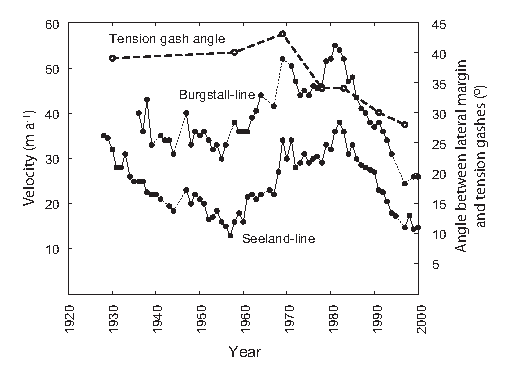
\includegraphics{72A712Fig01.eps}}
\caption{One-column figures should be $\leq$86$\,$mm.
Good artwork can make or break a paper. Capitalize
the first word of a label and use round not square 
brackets for units.}
\label{tracks}
\end{figure}

\subsubsection{Automatic references using \textsc{Bib}\upshape{\TeX}}

To generate automatic references from a bib database, you must first specify the database (we are using \verb"igsrefs.bib") and then the IGS bibliography style by placing the following two commands where you would like the references to appear (normally at the end of your paper, before \verb"\end{document}"):
\begin{verbatim}

\bibliography{igsrefs}
\bibliographystyle{igs}

\end{verbatim}
%
Then run through the following steps:
\begin{enumerate}
\item Run your paper through \LaTeX.
\item Run \textsc{Bib}\TeX\ on your paper.
\item Open the newly-created bbl file containing the cited references and copy the entire contents to just below the \verb"bibliography"/\verb"bibliographystyle" commands.
\item Then comment them out:
\begin{verbatim}
%\bibliography{igsrefs}
%\bibliographystyle{igs}
\end{verbatim}
\item Run your paper through \LaTeX\ \textit{twice} more. 
\end{enumerate}
The IGS do not need your bib or bbl files. Note that \textsc{Bib}\TeX\ will lose the second initial in the entry `Box JE', for example, if it has been typed as `\{J.E.\} Box' in the bib file. This is because any text in an entry enclosed in \{\,\} will be treated as a single unit, and will not be further parsed. Prof. Box's name will typeset correctly if entered as `J. E. Box' in the bib file. 

If you have cited 16 references from the bib database, e.g. 
\citep{Rignot08},
\citep{Rignot08_2},
\citep{Motyka11},
\citep{Morlighem10},
\citep{Morlighem11},
\citep{Seroussi11},
\citep{Yan13},
\citep{Rogozhina12},
\citep{Hanna13},
\citep{Goelzer13},
\citep{Lucas12},
\citep{Edwards14},
\citep{gladstone_grl_10},
\citep{Morlighem13},
\citep{Goldberg11} and
\citep{paterson94}, the output will be just those 16 references and they will appear at the end of the article.

\paragraph{Citations using natbib commands}
Note that the standard natbib style file has been modified to fall into line with IGS style. The modified style file is called igsnatbib.sty (included in this distribution), and works exactly the same as natbib.sty. The default IGS house style is \citep{Yan13}. The following combinations are also available -- refer to the natbib documentation if you require any further explanation:\\*[0.5\baselineskip]
\begin{tabular}{@{}l@{\hskip -94pt}l}
\citep{Yan13}
    & \verb"\citep{Yan13}"\\
\citep[see][p.$\,$34]{Yan13}\\
    & \verb"\citep[see][p.$\,$34]{Yan13}"\\
\citep[e.g.][]{Yan13}
    & \verb"\citep[e.g.][]{Yan13}"\\
\citep[Section~2.3]{Yan13}\\
    & \verb"\citep[Section~2.3]{Yan13}"\\
\citep{Yan13, Edwards14}\\
    &  \verb"\citep{Yan13, Edwards14}"\\
\cite{Yan13, Edwards14}\\
    &  \verb"\cite{Yan13, Edwards14}"\\
\citealt{Yan13}
    & \verb"\citealt{Yan13}"\\
\cite{Yan13}
    & \verb"\cite{Yan13}"\\
\citealp{Yan13}
    & \verb"\citealp{Yan13}"\\
\citeauthor{Yan13}
    & \verb"\citeauthor{Yan13}"\\
\citeyearpar{Yan13}
    & \verb"\citeyearpar{Yan13}"\\
\citeyear{Yan13}
    & \verb"\citeyear{Yan13}"
\end{tabular}

\begin{figure*}%fig2, two column
\centering{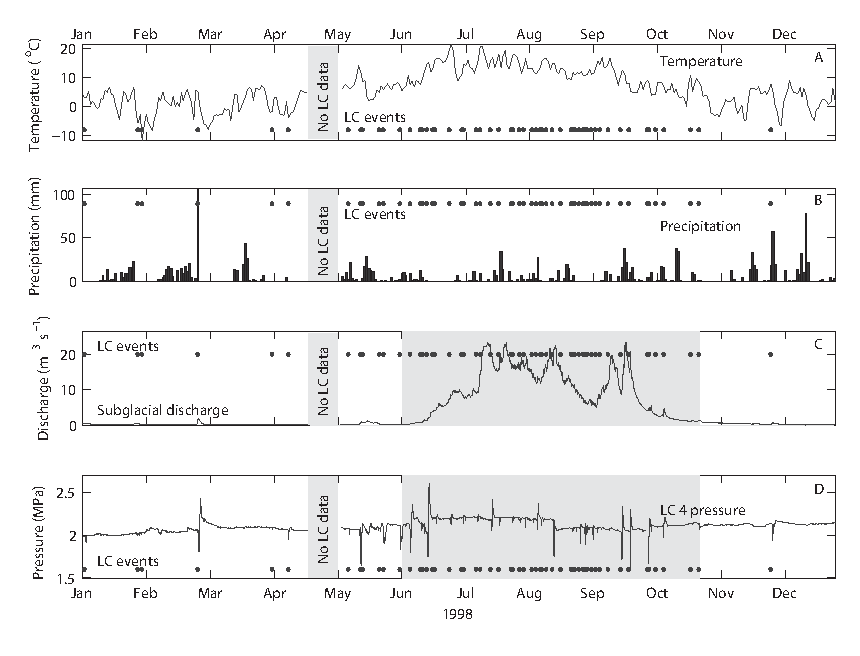
\includegraphics{72A712Fig02.eps}}
\caption{Two-column figures should be $\leq$178$\,$mm. SSA reconstructed components found by 
  projecting the SSA filters found using the whole 2000 traces in Fig.~4, on trace number 1, 
  ordered by magnitude of variance accounted for in the radar trace.}
\label{filters}
\vspace\baselineskip\hrule % to separate figure from verbatim
\vspace\baselineskip
\begin{verbatim}
\begin{figure*}%fig2, two column
\centering{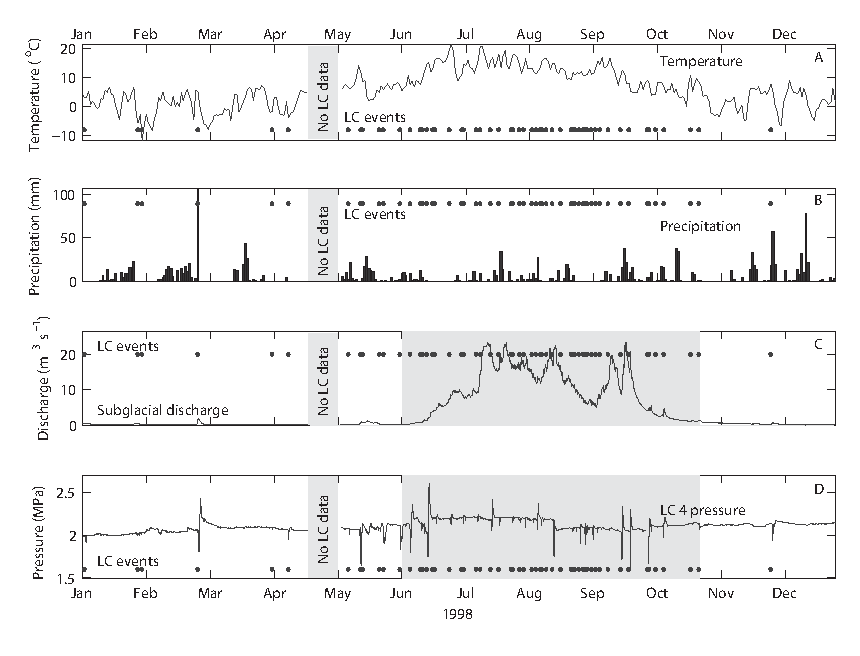
\includegraphics{72A712Fig02.eps}}
\caption{Two-column figures should be $\leq$178$\,$mm. SSA reconstructed components found by 
  projecting the SSA filters found using the whole 2000 traces in Fig.~4, on trace number 1, 
  ordered by magnitude of variance accounted for in the radar trace.}
\label{filters}
\end{figure*}
\end{verbatim}
\vspace\baselineskip\hrule % to separate verbatim from text
\end{figure*}


\section{Acknowledgements} 
We would like to thank Jason Amundson, Ed Bueler, Andrew Clifton, Gwenn~Flowers, Ralf Greve and Doug MacAyeal for their constructive reviews of the IGS class file and guide. Thanks are also due to Patrick Daly who once again helped to generate the latest version of igs.bst.

% authors generating their own bbl file would uncomment the following two lines, and comment out/delete the references below:

\bibliography{igsrefs}   % reads igsrefs.bib
\bibliographystyle{igs}  % imposes IGS bibliography style on output


\appendix
\section{Appendix}

Start an appendix by \hbox{typing \verb"\appendix\section{Appendix}".} Appendices appear after the references. Equation numbers automatically start again with (\ref{appeqn}).
\begin{equation}
\label{appeqn}
 2\eta\kappa \frac{\partial \skew1\bar u}{\partial t} + \rho_{\mathrm r} g \skew1\bar u + D\kappa^4 \skew1\bar u = \skew3\bar\sigma_{zz}.
\end{equation}

\section{Handling more than one appendix}
Use the following code to achieve heading APPENDIX~A followed by APPENDIX~B and APPENDIX~C, with appropriate equation numbers:

\begin{verbatim}

\appendix
\section{Appendix A}

\setcounter{equation}{0}
\renewcommand\theequation{B\arabic{equation}}
\section{Appendix B}

\setcounter{equation}{0}
\renewcommand\theequation{C\arabic{equation}}
\section{Appendix C}
\end{verbatim}

\end{document}
